\begin{activity}{Oceanic Lithosphere: Half-Space and Plate Cooling}

\section*{Purpose}
Newly formed oceanic lithosphere cools as it moves away from a ridge, and that cooling leaves two independent, measurable fingerprints: surface heat flow and seafloor depth. This activity derives both from the half-space cooling solution, shows why each becomes linear in a particular transformed variable, and tests the model against real global compilations -- including where it breaks.

\section*{Learning Outcomes}
By the end of this activity, you should be able to:
\begin{itemize}
  \item Derive surface heat flow and subsidence from the half-space cooling solution $T(z,t)$.
  \item Explain why $q^{-2}$ is linear in age and why depth is linear in $\sqrt{\text{age}}$, for a half-space.
  \item Identify where real oceanic data does and does not follow this prediction, and connect any departure to the plate cooling model's finite basal boundary condition.
  \item Relate the timescale at which half-space and plate predictions diverge to the characteristic time $\tau=L^2/\kappa$.
\end{itemize}

\section*{Background}
The half-space cooling solution, with $T(0,t)=T_0$ and $T(z,0)=T_m$ for all $z>0$, is
\[
T(z,t) = T_0 + (T_m-T_0)\,\erf\!\left(\frac{z}{2\sqrt{\kappa t}}\right).
\]
This is the same solution from Activity 9.A, now applied with $T_0$ as the seafloor (bottom water) temperature and $T_m$ as the mantle temperature it cools from.

\emph{Aside:} oceanic lithosphere technically forms by seafloor spreading, the $\gamma=1$ limit of the rifting model in your notes and problem set -- that limit is singular in the pure-shear formulation and requires a separate treatment, given in your notes. We do not need it here; the half-space and plate solutions below are self-contained.

\section*{Tasks}
\begin{questions}

\question{Deriving Surface Heat Flow}

Using $q_0(t) = k\left.\dfrac{\partial T}{\partial z}\right|_{z=0}$ and the chain rule, along with $\dfrac{d}{dx}\erf(x) = \dfrac{2}{\sqrt\pi}e^{-x^2}$, derive an expression for $q_0(t)$.

\answerbox[4cm]

You should arrive at $q_0(t) = \dfrac{k(T_m-T_0)}{\sqrt{\pi\kappa t}}$.

\question{Deriving Subsidence}

Thermal contraction of the cooling column, balanced isostatically against the water that fills the space it vacates, produces subsidence
\[
s(t) = \frac{\rho_m}{\rho_m-\rho_w}\,\alpha\int_0^\infty\bigl[T(z,0)-T(z,t)\bigr]\,dz.
\]

\begin{enumerate}[label=(\alph*)]
  \item Write $T(z,0)-T(z,t)$ in terms of the complementary error function, $\erfc(\eta)=1-\erf(\eta)$.
  \answerbox[2cm]

  \item Substitute $\eta=z/(2\sqrt{\kappa t})$ to change variables in the integral. You will need the identity $\displaystyle\int_0^\infty \erfc(\eta)\,d\eta = \frac{1}{\sqrt\pi}$ (given -- this one isn't worth re-deriving here).
  \answerbox[3cm]

  \item Combine your results to arrive at $s(t)$.
  \answerbox[2cm]
\end{enumerate}

You should arrive at $s(t) = \dfrac{2\rho_m\alpha(T_m-T_0)}{\rho_m-\rho_w}\sqrt{\dfrac{\kappa t}{\pi}}$.

\question{Why These Linearize}

\begin{enumerate}[label=(\alph*)]
  \item Using your result from Question 1, show that $q_0^{-2}$ is linear in $t$.
  \answerbox[2.5cm]

  \item Using your result from Question 2, in what variable is $s(t)$ linear?
  \answerbox[1.5cm]
\end{enumerate}

\question{Estimating the Fit Constants by Hand}

Write the half-space predictions as $q(t) = c_q/\sqrt{t}$ and $s(t) = c_s\sqrt{t}$, absorbing all the physical constants ($k$, $\kappa$, $T_m-T_0$, $\rho_m$, $\alpha$, ...) into the single constants $c_q$ and $c_s$. Two real data points from each dataset are given below; $s$ is depth relative to the ridge-depth reference of 2500~m.

\begin{center}
\begin{tabular}{ccc}
\toprule
\multicolumn{3}{c}{Heat flow} \\
$t$ (Ma) & $q$ (mW m$^{-2}$) & \\
\midrule
19.8  & 114.0 & \\
51.3  & 72.1  & \\
\bottomrule
\end{tabular}
\qquad
\begin{tabular}{ccc}
\toprule
\multicolumn{3}{c}{Bathymetry} \\
$t$ (Ma) & depth (m) & $s=$depth$-2500$ (m) \\
\midrule
11.3  & 3633 & \\
41.3  & 4633 & \\
\bottomrule
\end{tabular}
\end{center}

\begin{enumerate}[label=(\alph*)]
  \item Using $q(t)=c_q/\sqrt{t}$, compute $c_q$ from each heat flow point separately. Are your two estimates consistent with each other?
  \answerbox[2.5cm]

  \item Using $s(t)=c_s\sqrt{t}$, compute $c_s$ from each bathymetry point separately. Are your two estimates consistent with each other?
  \answerbox[2.5cm]

  \item Which pair of estimates agreed more closely -- $c_q$ or $c_s$? Given what generates scatter in young oceanic heat flow, suggest why one dataset might let a small number of points pin down its constant more reliably than the other.
  \answerbox[2.5cm]
\end{enumerate}

\question{Real Data: Heat Flow}

\begin{figure}[h]
    \centering
    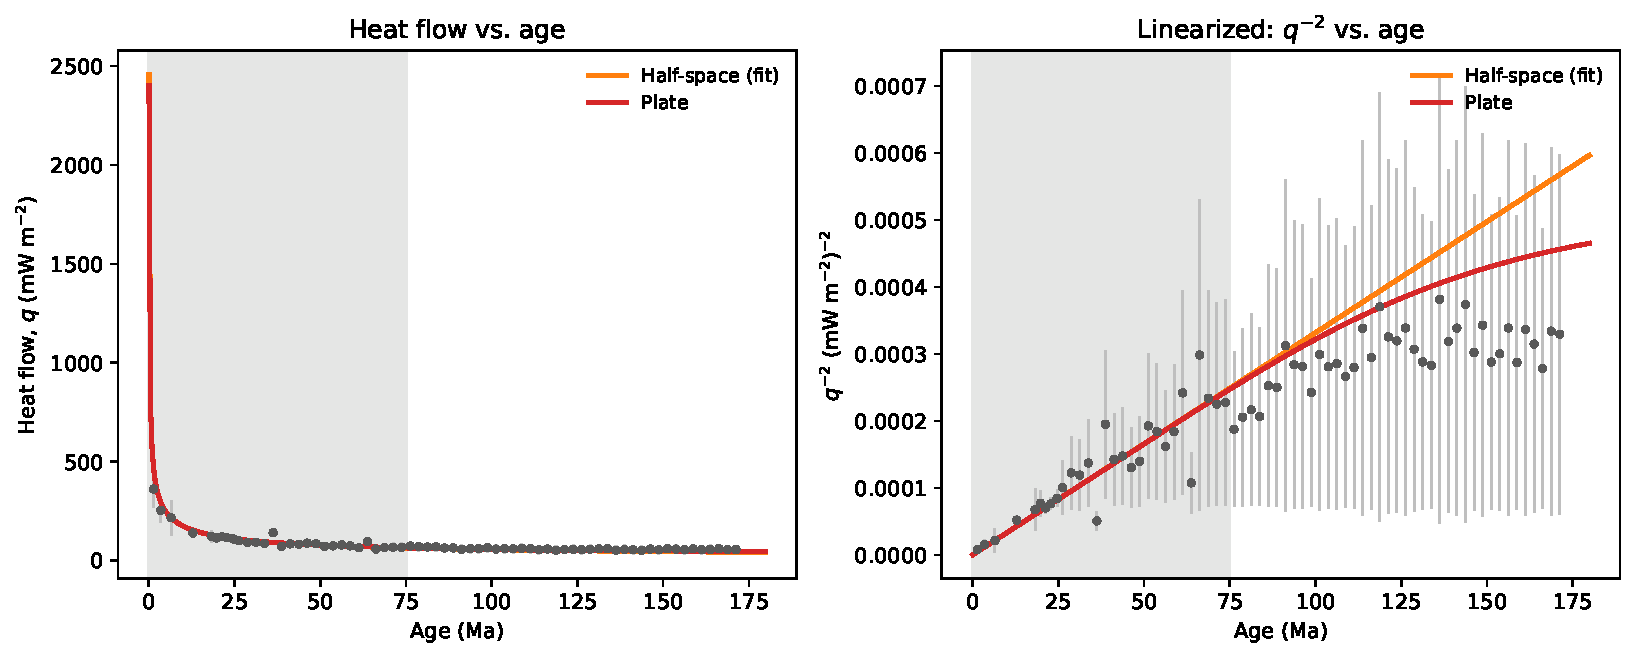
\includegraphics[width=\textwidth]{figures/9c_heatflow_age.pdf}
    \caption{Sediment-corrected global heat flow vs.\ seafloor age (binned, error bars show one standard deviation). The half-space curve here is fit by least squares to \emph{every} point in the shaded region ($t<75$~Ma), giving $c_q\approx549$~mW\,m$^{-2}$\,Ma$^{1/2}$.}
\end{figure}

\begin{enumerate}[label=(\alph*)]
  \item How does the full-dataset fit, $c_q\approx549$, compare to your two hand estimates from Question 4? Does this change how much you'd trust a constant estimated from just one or two points?
  \answerbox[2.5cm]

  \item At young ages, does the data sit above, below, or on the half-space prediction? What physical process, not included in this conductive model, might explain that?
  \answerbox[2.5cm]

  \item At the oldest ages shown, do half-space and plate predictions still agree closely, or have they begun to separate? What does that tell you about how old the seafloor needs to be before the two models are distinguishable in heat flow alone?
  \answerbox[2.5cm]
\end{enumerate}

\question{Real Data: Bathymetry}

\begin{figure}[h]
    \centering
    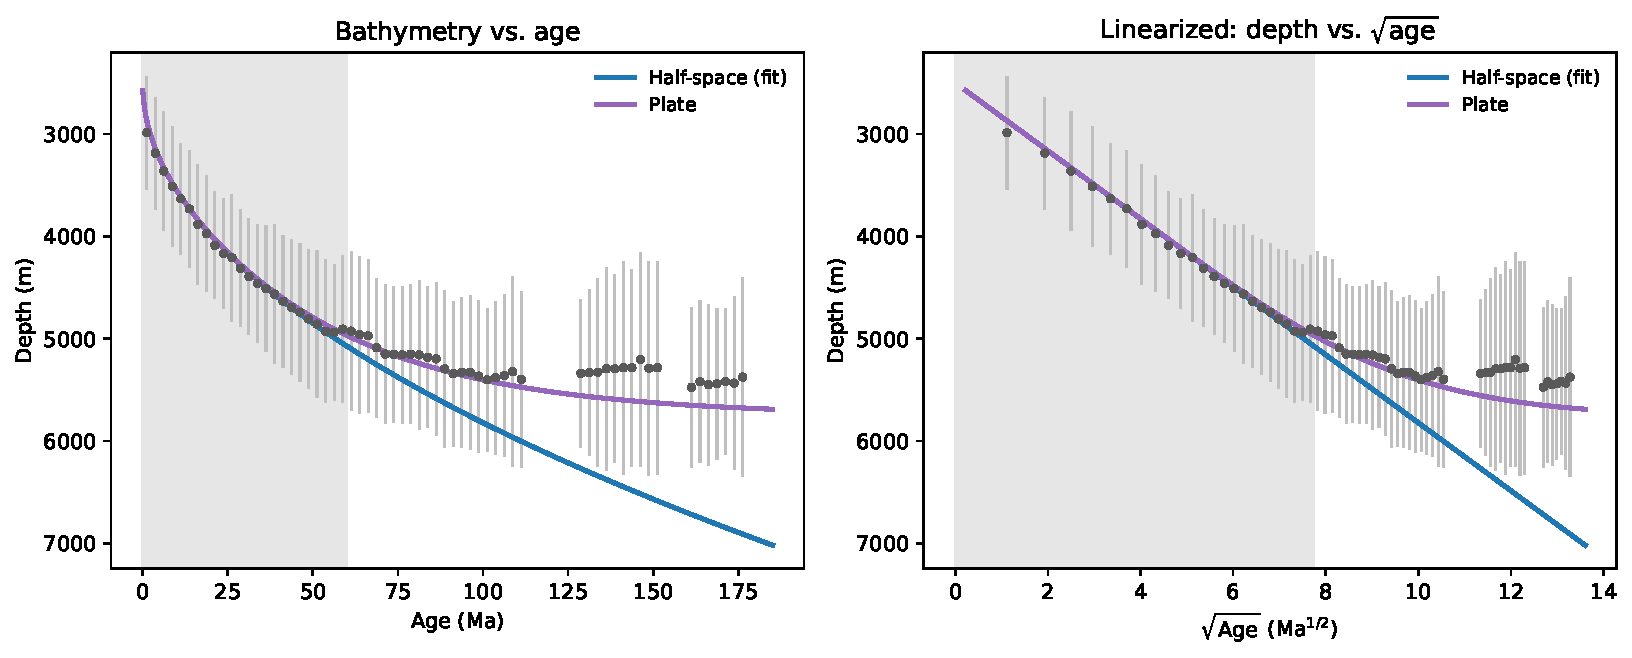
\includegraphics[width=\textwidth]{figures/9c_bathymetry_age.pdf}
    \caption{Global bathymetry vs.\ seafloor age (binned, error bars show one standard deviation). The half-space curve is fit to every point in the shaded region ($t<60$~Ma), giving $c_s\approx332$~m\,Ma$^{-1/2}$.}
\end{figure}

\begin{enumerate}[label=(\alph*)]
  \item How does this full-dataset fit compare to your two hand estimates from Question 4? Is the improvement from using more points as large as it was for heat flow?
  \answerbox[2cm]

  \item Compare this figure to Question 5's heat flow figure. In which observable does the half-space model's failure become obvious sooner, as a function of age?
  \answerbox[2.5cm]

  \item The half-space model has no plate thickness $L$ in it at all -- it's a model of infinite depth. Explain, physically, why real subsidence eventually stops following the half-space prediction.
  \answerbox[2.5cm]
\end{enumerate}

\question{Early and Late Time}

The characteristic time for the plate model is $\tau=L^2/\kappa$.

\begin{enumerate}[label=(\alph*)]
  \item For $t\ll\tau$, the plate solution reduces to the half-space solution. Why does a finite-thickness plate behave like an infinite half-space when it's young?
  \answerbox[2cm]

  \item For $t\gg\tau$, heat flow approaches a constant, $q_0\to k(T_m-T_0)/L$ -- independent of $t$. Why does the plate's finite thickness impose a floor on how thin the thermal boundary layer can get, when a half-space's doesn't?
  \answerbox[2.5cm]
\end{enumerate}

\end{questions}

\section*{Key Ideas}

\textbf{The same solution predicts two independent, testable observables.} Heat flow comes from the temperature gradient at the surface; subsidence comes from integrating the temperature deficit through the whole column. Both derive from the same $T(z,t)$, but they linearize in different variables ($t$ vs.\ $\sqrt t$) and, as you saw, they reveal the half-space model's breakdown at different ages.

\textbf{A model with no built-in length scale cannot predict its own failure.} The half-space solution has no plate thickness in it, so nothing internal to the model signals when it stops applying -- that only becomes visible by comparing to real data, or to a model (plate cooling) that does have a length scale.

\textbf{Early-time agreement between two models doesn't guarantee late-time agreement.} The plate and half-space solutions coincide for $t\ll\tau$ by construction, not by coincidence -- and diverge once the finite basal boundary condition is actually felt, at $t\sim\tau$.

\end{activity}
